\documentclass[]{article}
\usepackage{lmodern}
\usepackage{amssymb,amsmath}
\usepackage{ifxetex,ifluatex}
\usepackage{fixltx2e} % provides \textsubscript
\ifnum 0\ifxetex 1\fi\ifluatex 1\fi=0 % if pdftex
  \usepackage[T1]{fontenc}
  \usepackage[utf8]{inputenc}
\else % if luatex or xelatex
  \ifxetex
    \usepackage{mathspec}
  \else
    \usepackage{fontspec}
  \fi
  \defaultfontfeatures{Ligatures=TeX,Scale=MatchLowercase}
\fi
% use upquote if available, for straight quotes in verbatim environments
\IfFileExists{upquote.sty}{\usepackage{upquote}}{}
% use microtype if available
\IfFileExists{microtype.sty}{%
\usepackage{microtype}
\UseMicrotypeSet[protrusion]{basicmath} % disable protrusion for tt fonts
}{}
\usepackage[margin=1in]{geometry}
\usepackage{hyperref}
\hypersetup{unicode=true,
            pdftitle={UVC datasets - exploring monitoring structure and herbivore assemblages},
            pdfborder={0 0 0},
            breaklinks=true}
\urlstyle{same}  % don't use monospace font for urls
\usepackage{color}
\usepackage{fancyvrb}
\newcommand{\VerbBar}{|}
\newcommand{\VERB}{\Verb[commandchars=\\\{\}]}
\DefineVerbatimEnvironment{Highlighting}{Verbatim}{commandchars=\\\{\}}
% Add ',fontsize=\small' for more characters per line
\usepackage{framed}
\definecolor{shadecolor}{RGB}{248,248,248}
\newenvironment{Shaded}{\begin{snugshade}}{\end{snugshade}}
\newcommand{\KeywordTok}[1]{\textcolor[rgb]{0.13,0.29,0.53}{\textbf{#1}}}
\newcommand{\DataTypeTok}[1]{\textcolor[rgb]{0.13,0.29,0.53}{#1}}
\newcommand{\DecValTok}[1]{\textcolor[rgb]{0.00,0.00,0.81}{#1}}
\newcommand{\BaseNTok}[1]{\textcolor[rgb]{0.00,0.00,0.81}{#1}}
\newcommand{\FloatTok}[1]{\textcolor[rgb]{0.00,0.00,0.81}{#1}}
\newcommand{\ConstantTok}[1]{\textcolor[rgb]{0.00,0.00,0.00}{#1}}
\newcommand{\CharTok}[1]{\textcolor[rgb]{0.31,0.60,0.02}{#1}}
\newcommand{\SpecialCharTok}[1]{\textcolor[rgb]{0.00,0.00,0.00}{#1}}
\newcommand{\StringTok}[1]{\textcolor[rgb]{0.31,0.60,0.02}{#1}}
\newcommand{\VerbatimStringTok}[1]{\textcolor[rgb]{0.31,0.60,0.02}{#1}}
\newcommand{\SpecialStringTok}[1]{\textcolor[rgb]{0.31,0.60,0.02}{#1}}
\newcommand{\ImportTok}[1]{#1}
\newcommand{\CommentTok}[1]{\textcolor[rgb]{0.56,0.35,0.01}{\textit{#1}}}
\newcommand{\DocumentationTok}[1]{\textcolor[rgb]{0.56,0.35,0.01}{\textbf{\textit{#1}}}}
\newcommand{\AnnotationTok}[1]{\textcolor[rgb]{0.56,0.35,0.01}{\textbf{\textit{#1}}}}
\newcommand{\CommentVarTok}[1]{\textcolor[rgb]{0.56,0.35,0.01}{\textbf{\textit{#1}}}}
\newcommand{\OtherTok}[1]{\textcolor[rgb]{0.56,0.35,0.01}{#1}}
\newcommand{\FunctionTok}[1]{\textcolor[rgb]{0.00,0.00,0.00}{#1}}
\newcommand{\VariableTok}[1]{\textcolor[rgb]{0.00,0.00,0.00}{#1}}
\newcommand{\ControlFlowTok}[1]{\textcolor[rgb]{0.13,0.29,0.53}{\textbf{#1}}}
\newcommand{\OperatorTok}[1]{\textcolor[rgb]{0.81,0.36,0.00}{\textbf{#1}}}
\newcommand{\BuiltInTok}[1]{#1}
\newcommand{\ExtensionTok}[1]{#1}
\newcommand{\PreprocessorTok}[1]{\textcolor[rgb]{0.56,0.35,0.01}{\textit{#1}}}
\newcommand{\AttributeTok}[1]{\textcolor[rgb]{0.77,0.63,0.00}{#1}}
\newcommand{\RegionMarkerTok}[1]{#1}
\newcommand{\InformationTok}[1]{\textcolor[rgb]{0.56,0.35,0.01}{\textbf{\textit{#1}}}}
\newcommand{\WarningTok}[1]{\textcolor[rgb]{0.56,0.35,0.01}{\textbf{\textit{#1}}}}
\newcommand{\AlertTok}[1]{\textcolor[rgb]{0.94,0.16,0.16}{#1}}
\newcommand{\ErrorTok}[1]{\textcolor[rgb]{0.64,0.00,0.00}{\textbf{#1}}}
\newcommand{\NormalTok}[1]{#1}
\usepackage{graphicx,grffile}
\makeatletter
\def\maxwidth{\ifdim\Gin@nat@width>\linewidth\linewidth\else\Gin@nat@width\fi}
\def\maxheight{\ifdim\Gin@nat@height>\textheight\textheight\else\Gin@nat@height\fi}
\makeatother
% Scale images if necessary, so that they will not overflow the page
% margins by default, and it is still possible to overwrite the defaults
% using explicit options in \includegraphics[width, height, ...]{}
\setkeys{Gin}{width=\maxwidth,height=\maxheight,keepaspectratio}
\IfFileExists{parskip.sty}{%
\usepackage{parskip}
}{% else
\setlength{\parindent}{0pt}
\setlength{\parskip}{6pt plus 2pt minus 1pt}
}
\setlength{\emergencystretch}{3em}  % prevent overfull lines
\providecommand{\tightlist}{%
  \setlength{\itemsep}{0pt}\setlength{\parskip}{0pt}}
\setcounter{secnumdepth}{0}
% Redefines (sub)paragraphs to behave more like sections
\ifx\paragraph\undefined\else
\let\oldparagraph\paragraph
\renewcommand{\paragraph}[1]{\oldparagraph{#1}\mbox{}}
\fi
\ifx\subparagraph\undefined\else
\let\oldsubparagraph\subparagraph
\renewcommand{\subparagraph}[1]{\oldsubparagraph{#1}\mbox{}}
\fi

%%% Use protect on footnotes to avoid problems with footnotes in titles
\let\rmarkdownfootnote\footnote%
\def\footnote{\protect\rmarkdownfootnote}

%%% Change title format to be more compact
\usepackage{titling}

% Create subtitle command for use in maketitle
\newcommand{\subtitle}[1]{
  \posttitle{
    \begin{center}\large#1\end{center}
    }
}

\setlength{\droptitle}{-2em}
  \title{UVC datasets - exploring monitoring structure and herbivore assemblages}
  \pretitle{\vspace{\droptitle}\centering\huge}
  \posttitle{\par}
  \author{}
  \preauthor{}\postauthor{}
  \date{}
  \predate{}\postdate{}


\begin{document}
\maketitle

\paragraph{Seychelles}\label{seychelles}

\begin{itemize}
\tightlist
\item
  Seychelles data are 7m radius point counts conducted at 21 reef sites
  in 1994, 2005, 2008, 2011, 2014, 2017.
\item
  Sites were stratified according to habitat (granite = 7, patch = 7,
  carbonate = 7) and management status (12 = fished, 9 = MPAs)
\item
  Reefs are the inhabited Seychelles islands, Mahe and Praslin
\item
  Useful papers describing dataset methods: Graham et al. 2015
  (Predicting climate-driven regime shifts\ldots{}, Nature)
\end{itemize}

Across all surveys, \texttt{37} herbivore species were recorded, which
are composed of:

\begin{verbatim}
##                  FG species
## 1 Herbivore Browser       5
## 2  Herbivore Grazer      15
## 3 Herbivore Scraper      17
\end{verbatim}

Scrapers dominated herbivore assemblages on both fished and protected
reefs, and browser biomass was slightly higher than grazer biomass after
1994 (i.e.~after bleaching). High variability in browser biomass
suggests that strong spatial variation in browser presence. This was
less true for scrapers, for which biomass may be high at all reef sites.
There was a weak protection effect apparent, with slightly higher
biomass of all feeding groups in protected sites.

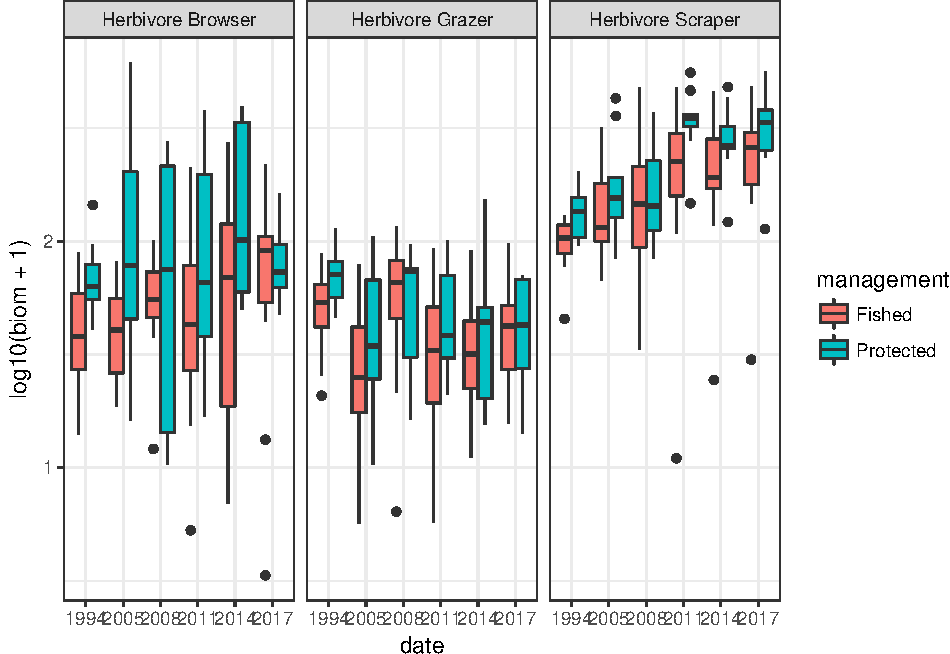
\includegraphics{UVC-datasets-explore_files/figure-latex/unnamed-chunk-3-1.pdf}

Grazer size distributions indicated high abundance of small-bodied
individuals. Scraper and browser sizes were more equitably distributed
across the size range. Scrapers had the largest body sizes, with some
individuals between 0.5-2 kg.

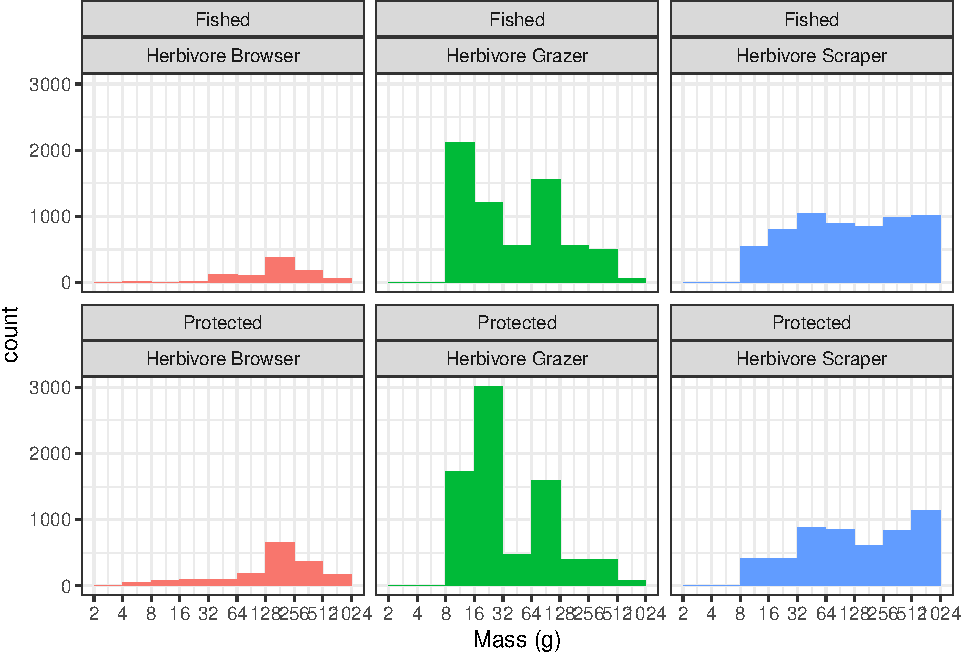
\includegraphics{UVC-datasets-explore_files/figure-latex/unnamed-chunk-4-1.pdf}

\textbf{Common herbivore species}

Considering common species as those that are high in abundance or
biomass (i.e.~mean biomass across UVC replicates at each site).

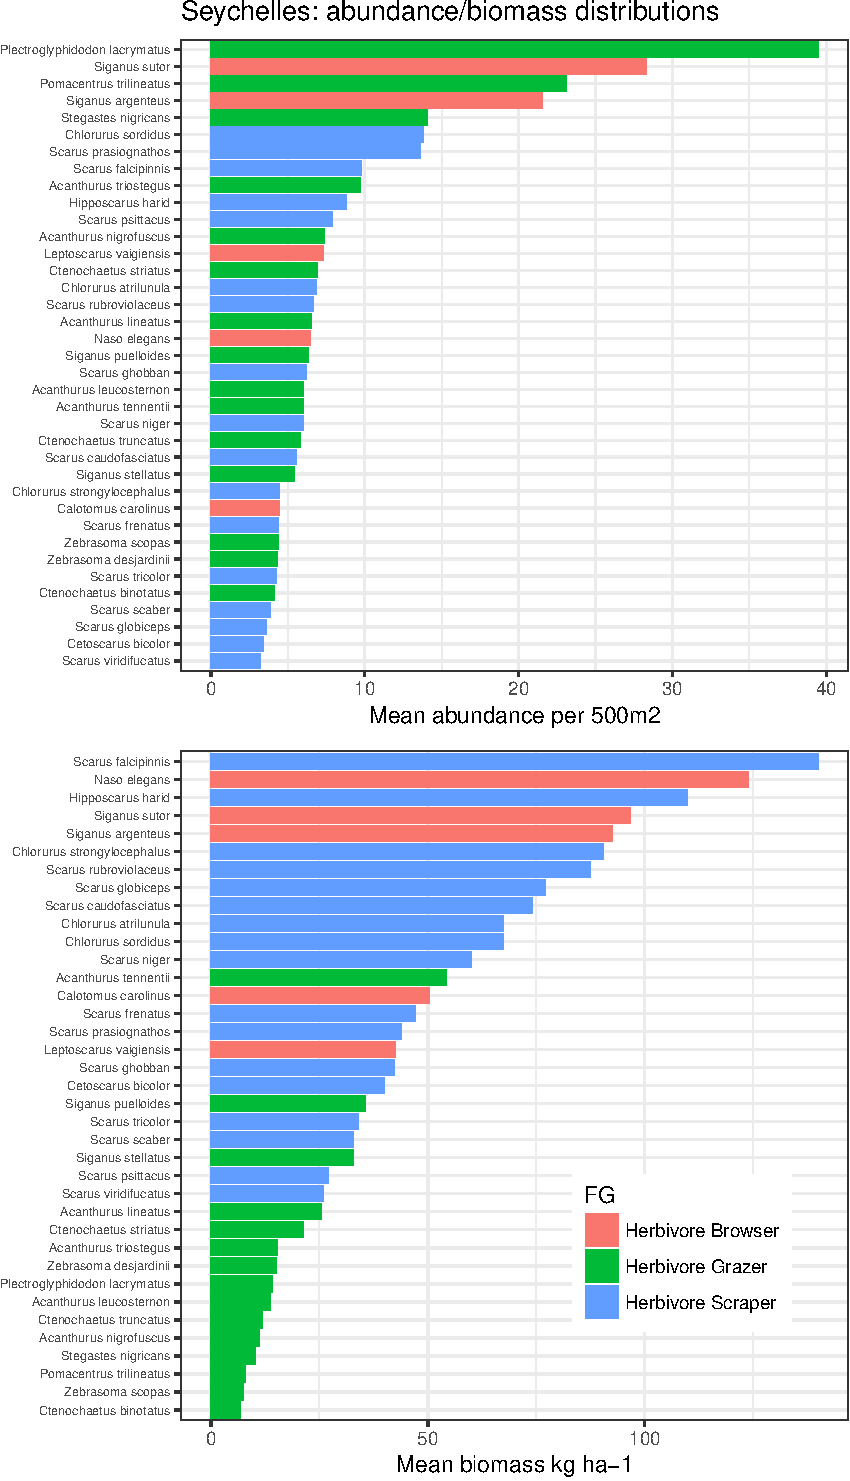
\includegraphics{UVC-datasets-explore_files/figure-latex/unnamed-chunk-5-1.pdf}

\paragraph{Maldives}\label{maldives}

\begin{itemize}
\tightlist
\item
  11 sampled sites
\item
  4 transects each site of 250 m\^{}2 (most) or 100 m\^{}2 area
\item
  1 depth level (8m)
\item
  1 management level (Fished)
\item
  1 habitat level (Exposed)
\item
  30 herbivore species (3 browser spp., 13 grazer spp., 14 scraper spp.)
\item
  7 herbivore families
\end{itemize}

\section{biomass ditribution across functional
groups}\label{biomass-ditribution-across-functional-groups}

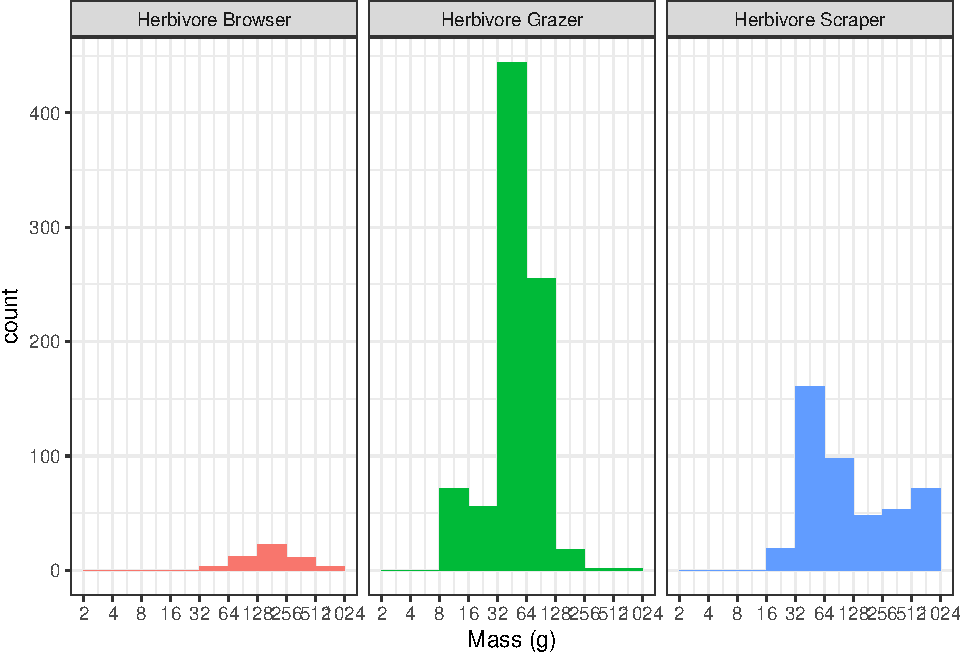
\includegraphics{UVC-datasets-explore_files/figure-latex/unnamed-chunk-6-1.pdf}
*Browsers few but large, grazers smaller but many, scrapers more equally
spread in both

\section{common herbivore species}\label{common-herbivore-species}

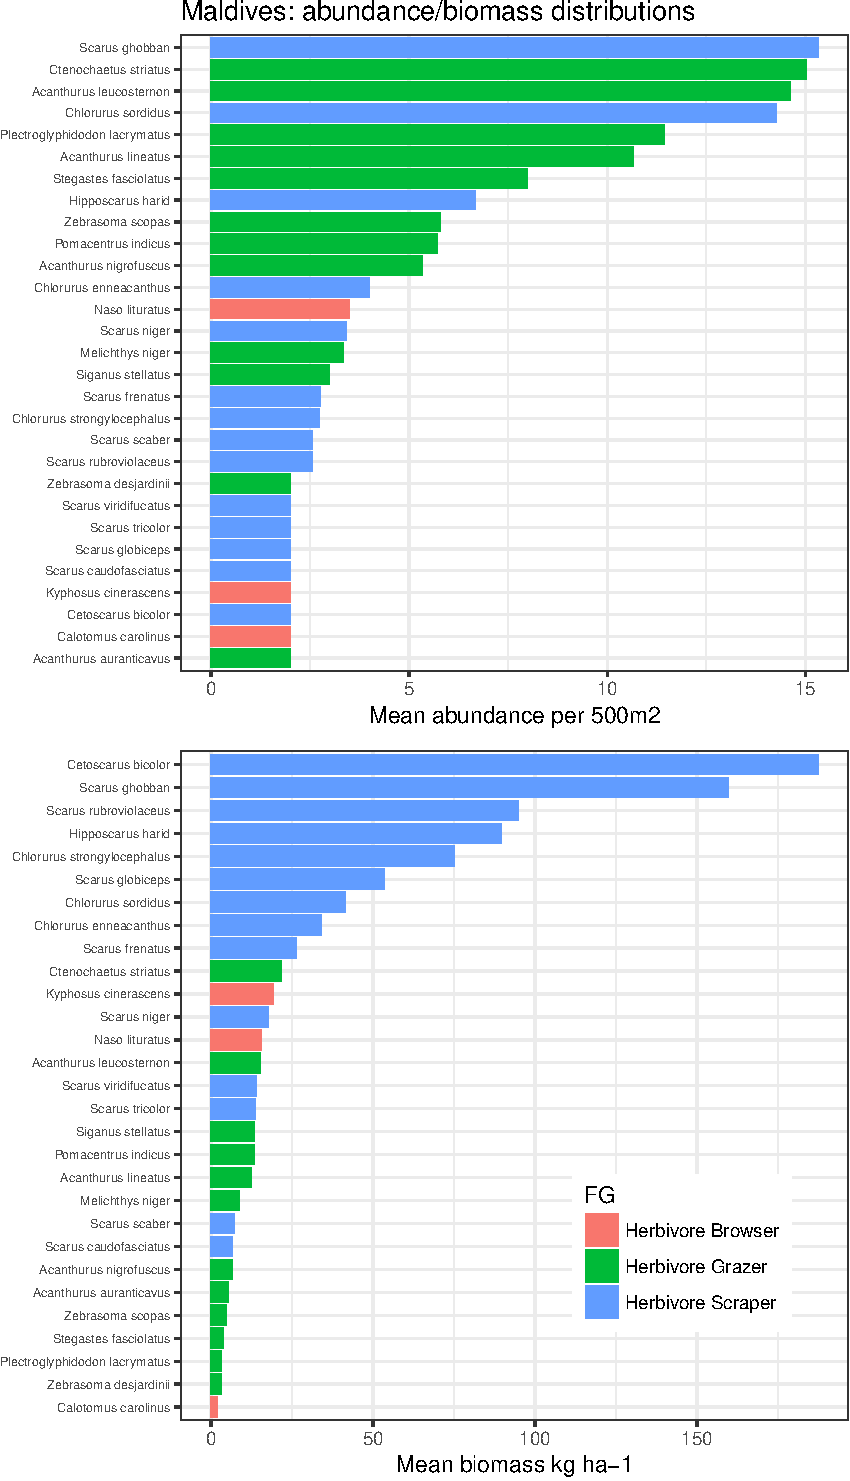
\includegraphics{UVC-datasets-explore_files/figure-latex/unnamed-chunk-7-1.pdf}

\paragraph{GBR}\label{gbr}

\begin{itemize}
\tightlist
\item
  Nov 2010 \& Jan 2011
\item
  5 reefs, 3 sites each, 4 transects each of 250 m\^{}2 (most) or 100
  m\^{}2 area
\item
  1 management level (fished)
\item
  18 habitat levels (3 exposed, 3 sheltered, crossed with
  crest-flat-slope)
\item
  NA depth
\item
  8 herbivore families
\item
  71 species (10 browser spp., 40 grazer spp., 21 scraper spp.)
\end{itemize}

\begin{Shaded}
\begin{Highlighting}[]
\KeywordTok{library}\NormalTok{(ggplot2)}
\KeywordTok{library}\NormalTok{(tidyverse)}

\KeywordTok{load}\NormalTok{(}\StringTok{'data/wio_gbr_herb_master.Rdata'}\NormalTok{)}
\NormalTok{gbr <-}\StringTok{ }\NormalTok{herb }\OperatorTok\StringTok{ }\KeywordTok{filter}\NormalTok{(dataset}\OperatorTok{==}\StringTok{'GBR'}\NormalTok{)}
\end{Highlighting}
\end{Shaded}

\section{biomass by functional group}\label{biomass-by-functional-group}

\includegraphics{UVC-datasets-explore_files/figure-latex/unnamed-chunk-9-1.pdf}

\section{common species}\label{common-species}

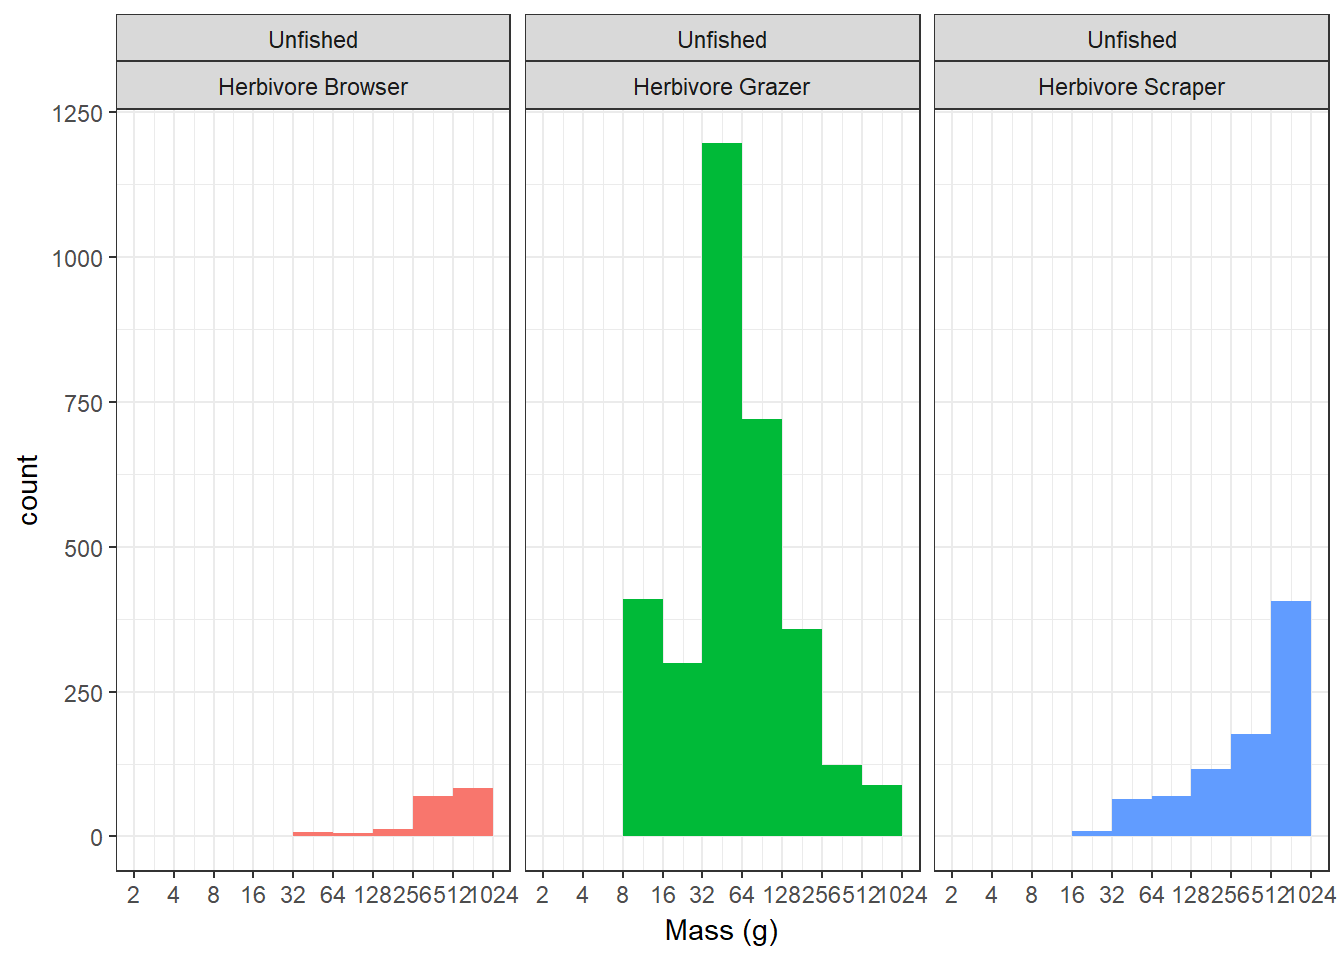
\includegraphics{UVC-datasets-explore_files/figure-latex/unnamed-chunk-10-1.pdf}
\includegraphics{UVC-datasets-explore_files/figure-latex/unnamed-chunk-10-2.pdf}
\#ugly biomass gradient across habitat for later

\begin{Shaded}
\begin{Highlighting}[]
\KeywordTok{ggplot}\NormalTok{(gbr, }\KeywordTok{aes}\NormalTok{(}\KeywordTok{log}\NormalTok{(mass.g, }\DecValTok{2}\NormalTok{), }\DataTypeTok{fill=}\NormalTok{FG)) }\OperatorTok{+}\StringTok{ }\KeywordTok{geom_histogram}\NormalTok{(}\DataTypeTok{breaks=}\KeywordTok{c}\NormalTok{(}\DecValTok{1}\OperatorTok{:}\DecValTok{10}\NormalTok{)) }\OperatorTok{+}\StringTok{ }
\StringTok{  }\KeywordTok{facet_wrap}\NormalTok{(habitat}\OperatorTok{~}\NormalTok{FG) }\OperatorTok{+}\StringTok{ }\KeywordTok{theme}\NormalTok{(}\DataTypeTok{legend.position=}\StringTok{'none'}\NormalTok{) }\OperatorTok{+}\StringTok{ }
\StringTok{  }\KeywordTok{scale_x_continuous}\NormalTok{(}\DataTypeTok{breaks=}\KeywordTok{c}\NormalTok{(}\DecValTok{1}\OperatorTok{:}\DecValTok{10}\NormalTok{), }\DataTypeTok{labels=}\KeywordTok{c}\NormalTok{(}\DecValTok{2}\OperatorTok{^}\KeywordTok{c}\NormalTok{(}\DecValTok{1}\OperatorTok{:}\DecValTok{10}\NormalTok{))) }\OperatorTok{+}\StringTok{ }\KeywordTok{labs}\NormalTok{ (}\DataTypeTok{x=}\StringTok{'Mass (g)'}\NormalTok{)}
\end{Highlighting}
\end{Shaded}

\includegraphics{UVC-datasets-explore_files/figure-latex/unnamed-chunk-11-1.pdf}

\paragraph{Chagos}\label{chagos}

\emph{Exploring the data}

Chagos dataset: total of 52 species, 5729 records, across 20 sites at 4
reefs, with between 1-4 transects at each site.

\begin{verbatim}
##                  FG species
## 1 Herbivore Browser       4
## 2  Herbivore Grazer      18
## 3 Herbivore Scraper      21
\end{verbatim}

Very few browser species (5) as compared to grazers (22) and scrapers
(25)\ldots{} but there are some duplicate species due to typos, so still
need to clean that up.

\includegraphics{UVC-datasets-explore_files/figure-latex/unnamed-chunk-16-1.pdf}
There are more grazers than any other functional group. Most grazers are
mid-sized, whereas there are more large scrapers and browsers. The mean
size of browzers is 1476g, grazers 115g, and scrapers 1808.

Now need to look at abundance and biomass of species and functional
groups across sites\ldots{}

\includegraphics{UVC-datasets-explore_files/figure-latex/unnamed-chunk-17-1.pdf}

\includegraphics{UVC-datasets-explore_files/figure-latex/unnamed-chunk-18-1.pdf}

There are no dates recorded for the Chagos dataset, so no time series
analyses could be done. Additionally, all of Chagos is ``unfished''.
Therefore, only ``depth'' and ``habitat'' gradients were explored
further to biomass. If lat long values can be attached to site names, a
spatial look at the data can be done as well.

\includegraphics{UVC-datasets-explore_files/figure-latex/unnamed-chunk-19-1.pdf}


\end{document}
